\documentclass[letter,11pt]{article}

\usepackage[spanish,es-nodecimaldot]{babel}
\usepackage[utf8]{inputenc}

\usepackage{lmodern}
\usepackage[T1]{fontenc}
\usepackage{textcomp}

\usepackage{framed}
\usepackage[svgnames]{xcolor}
\colorlet{shadecolor}{Gainsboro!50}

\usepackage[labelfont=bf]{caption}
\usepackage{graphicx}
\usepackage{pstricks}

\usepackage{anysize}
\marginsize{3cm}{2cm}{2cm}{3cm}

\usepackage{siunitx}
\usepackage{amsmath}
\usepackage{array}
\usepackage{alltt}

\usepackage{fancyhdr}
\usepackage{lastpage}
\pagestyle{fancy}
\fancyhf{}
\fancyhead[LE,RO]{Laboratorio de Física Básica III}
\fancyfoot[CO,CE]{\thepage\ de \pageref{LastPage}}

\special{papersize=215.9mm,279.4mm}

\usepackage[
    pdfauthor={
        Bastos Lizondo Rosemary;
        Blanco Alconz John Brandon;
        Caballero Burgoa Carlos Eduardo;
        Villena Gutiérrez Ismael Cristian
    },%
    pdftitle={Laboratorio de Física Básica III},%
    pdfsubject={Ley de Ohm y fuentes de tensión continua},%
    colorlinks,%
    citecolor=black,%
    filecolor=black,%
    linkcolor=black,%
    urlcolor=black,
    breaklinks]{hyperref}
\usepackage{breakurl}

\newcommand{\blankpage}{
\newpage
\thispagestyle{empty}
\mbox{}
\newpage
}

\renewcommand{\arraystretch}{1.2}

\begin{document}

\begin{titlepage}
\begin{center}
{\Large UNIVERSIDAD MAYOR DE SAN SIMÓN}\\
\vspace*{0.15cm}
{\large FACULTAD DE CIENCIAS Y TECNOLOGÍA}\\
\vspace*{0.10cm}
DEPARTAMENTO DE FÍSICA\\
\vspace*{3.0cm}
{\Large \textbf{LABORATORIO DE FÍSICA BÁSICA III}}\\
\vspace*{0.3cm}
{\Large \textbf{INFORME No. 3}}\\
\vspace*{3.5cm}
{\Large \textbf{LEY DE \emph{OHM} Y \\ FUENTES DE TENSIÓN CONTINUA}}\\
\end{center}

\vspace*{5.8cm}
\leftskip=7.95cm
\noindent
\textbf{Integrantes:}\\
Bastos Lizondo Rosemary.\\
Blanco Alconz John Brandon.\\
Caballero Burgoa Carlos Eduardo.\\
Villena Gutiérrez Ismael Cristian.\\
\newline
\textbf{Docente:}\\
Ing. Flores Flores, Freddy.\\
\newline
\textbf{Grupo:} G3.\\
\textbf{Fecha de entrega:} 07 de Abril del 2021.\\

\end{titlepage}

\section{Evaluación previa}
\begin{enumerate}
\item \textbf{¿Qué expresa ley de \emph{Ohm}?} \\
La ley de \emph{Ohm} establece que la cantidad de corriente que pasa por un
circuito es directamente proporcional al voltaje aplicado e inversamente
proporcional a la resistencia del circuito.

\item \textbf{¿Con qué instrumento se mide la corriente eléctrica y la
diferencia de potencial, y cómo se deben conectar para su medición?} \\
La intensidad de corriente eléctrica se mide colocando el instrumento sobre la
línea (fase) a la cual se desea medir. El método de conexión es en serie con la
carga, es decir, se conecta el instrumento sobre el mismo cable. Se utiliza un
amperímetro.

Para la medición de la diferencia de potencial se debe colocar el instrumento de
forma paralela a la carga o a la fuente. Se utiliza un voltímetro.

\item \textbf{¿Qué es la resistencia interna?} \\
Como una batería real está hecha de materia, dentro de la batería hay una
resistencia al flujo de carga eléctrica, esta resistencia se conoce como
resistencia interna.

\item \textbf{¿Qué valores deben tener las resistencias internas de los
voltímetros y amperímetros?} \\
La resistencia interna del voltímetro ha de ser al menos 10 veces mayor que la
resistencia cuya tensión se quiere medir, para que de esta forma el error
cometido no sea demasiado grande.

La resistencia interna del amperímetro ha de ser al menos 10 veces menor que la
resistencia del circuito que se quiere medir.

\item \textbf{¿Cuáles son las diferencias entre una fuente de tensión continua
ideal y una real?} \\
Una fuente de tensión real es la que tiene una determinada resistencia interna
($R_{i}$). En esta $R_{i}$, hay una pérdida de tensión. El resto de la
tensión va a la carga que es la que se aprovecha.

Una fuente de tensión ideal es la que tendría una $R_{i} = 0$ y producirá una
salida de tensión constante.

\item \textbf{¿Qué cuidados se tienen para el uso de una fuente de tensión
continua?} \\
Los equipos que trabajan con pilas o baterías, no representan, en general,
ningún riesgo para la vida humana; pero cuando hablamos de una red eléctrica,
tanto industrial como doméstica, tenemos que tomar cuidados importantes para no
recibir una descarga o shock eléctrico, esto también es valido para los voltajes
más bajos, como $110 V$.

Una regla general y a la cual tenemos que dar muchísima importancia, es que
antes de comenzar cualquier trabajo con electricidad de red, tanto en la
industria como en nuestras viviendas, es cortar el suministro de tensión,
accionando el dispositivo que tengamos a la entrada de corriente de la casa, o
del sector si se trata de una industria. Cualquiera que sea el protector
utilizado, hay que interrumpir en todos los casos el flujo de corriente
eléctrica.

\item \textbf{¿Qué es la fuerza electromotriz de una fuente, y en qué se
distingue con una diferencia de potencial?} \\
Cuando conectamos los bornes o polos de un generador eléctrico en un circuito se
rompe la estabilidad de las cargas y estas comienzan a moverse. El generador
está realizando un trabajo para impulsar las cargas aumentando su energía
potencial.

La capacidad que poseen los generadores para poner en movimiento las cargas se
mide mediante una magnitud denominada fuerza electromotriz (FEM).

La fuerza electromotriz ($\epsilon$) de un generador es el trabajo eléctrico que
realiza por cada unidad de carga positiva que lo atraviesa, aunque $\epsilon$ se
denomine fuerza electromotriz, no se trata de una fuerza, simplemente es la
causa de que se genere una diferencia de potencial.

\item \textbf{¿Qué es la corriente de cortocircuito?} \\
Un corto circuito es un fenómeno eléctrico que ocurre cuando dos puntos entre
los cuales existe una diferencia de potencial se ponen en contacto entre sí,
caracterizándose por elevadas corrientes circulantes hasta el punto de falla.
Se puede decir que un corto circuito es también el establecimiento de un flujo
de corriente eléctrica muy alta, debido a una conexión por un circuito de baja
impedancia, que prácticamente siempre ocurren por accidente. La magnitud de la
corriente de corto circuito es mucho mayor que la corriente nominal o de carga
que circula por el mismo.

El objetivo del estudio de corto circuito es calcular el valor máximo de la
corriente y su comportamiento durante el tiempo que permanece el mismo. Esto
permite determinar el valor de la corriente que debe interrumpirse y conocer el
esfuerzo al que son sometidos los equipos durante el tiempo transcurrido desde
que se presenta la falla hasta que se interrumpe la circulación de la corriente.
\end{enumerate}

\section{Objetivos}
\begin{itemize}
    \item Verificar la ley de Ohm.
    \item Encontrar la relación funcional entre la diferencia de potencial de
        los bornes de una fuente de tensión continua y la corriente que circula
        por el circuito.
    \item Determinar el valor de la fuerza electromotriz ($FEM$), la resistencia
        interna ($r_i$) y la corriente de cortocircuito ($I_{cc}$) de una fuente
        de tensión continua.
\end{itemize}

\section{Fundamento teórico}

\subsection{Ley de \emph{Ohm}}
La ley de \emph{Ohm} indica que la diferencia de potencial $V_{ab}$ entre los
extremos de un conductor es directamente proporcional a la corriente que circula
por él, donde la constante de proporcionalidad es la resistencia eléctrica que
el conductor tiene al paso de la corriente:

\begin{equation}
    V_{ab} = R \cdot I
\label{ohm}
\end{equation}

La unidad de medida de la resistencia eléctrica es el \emph{ohmio} [$\Omega$].

Para producir el movimiento de carga eléctrica (corriente eléctrica), los
extremos de la resistencia se conectan a una fuente de tensión.

\subsection{Fuente de tensión continua ideal}
Una fuente de tensión continua ideal, es aquella fuente que suministra una
diferencia de potencial $V_{ab}$ constante, para cualquier valor de la corriente
eléctrica que circula por el circuito, es decir, es independiente del valor de
la resistencia eléctrica $R$ del circuito.

\subsection{Fuente de tensión continua real}
Entre las fuentes de tensión continua real se tienen: pilas, baterías, fuentes
de alimentación con energía eléctrica, y se diferencia de una fuente de tensión
continua ideal por su resistencia interna (producida por el conjunto de piezas
de la fuente de tensión; conductores, soluciones ácidas, metales, etc.), que
está conectada en serie con la propia fuente de tensión. La diferencia de
potencial entre los bornes de la fuente de tensión, depende del valor de la
corriente eléctrica que circula por el circuito.

Aplicando la ley de voltaje de \emph{Kirchhoff}, el voltaje entre los puntos $a$
y $b$ del circuito es:

\begin{equation}
    V_{ab} = \epsilon - r_i \cdot I
\label{kirchhoff}
\end{equation}

Donde: $\epsilon$ es la $FEM$, y $r_i$ es la resistencia interna. Los valores
extremos para la resistencia eléctrica $R$ son: para $R = \infty$, se tiene un
circuito abierto, entonces la corriente en $R = 0$, entonces se tiene que:
$\epsilon = V_{ab}$. Para $R = 0$, se tiene un circuito en cortocircuito, los
bornes de la fuente de tensión están unidos a través de una conexión de
resistencia despreciable. La corriente de cortocircuito $I_{cc}$ es la máxima
posible:

\begin{equation}
    I_{cc} = \frac{e}{r_i}
\label{icc}
\end{equation}

\section{Materiales}
\begin{itemize}
\item Simulador «PhET Interactive Simulations» Kit de Construcción de Circuitos:
CD - Laboratorio Virtual.
\end{itemize}

\section{Procedimiento experimental}

\subsection{Ley de \emph{Ohm}}
A continuación se describe el procedimiento experimental que se llevará a cabo.

\begin{enumerate}
\item Ir al simulador ubicado en la dirección web:
(https://phet.colorado.edu/sims/html/circuit-construction-kit-dc-virtual-lab/latest/circuit-construction-kit-dc-virtual-lab\_es.html),
tal como se muestra en la \textbf{Figura \ref{figura1}}.

\begin{figure}[!h]
\centering
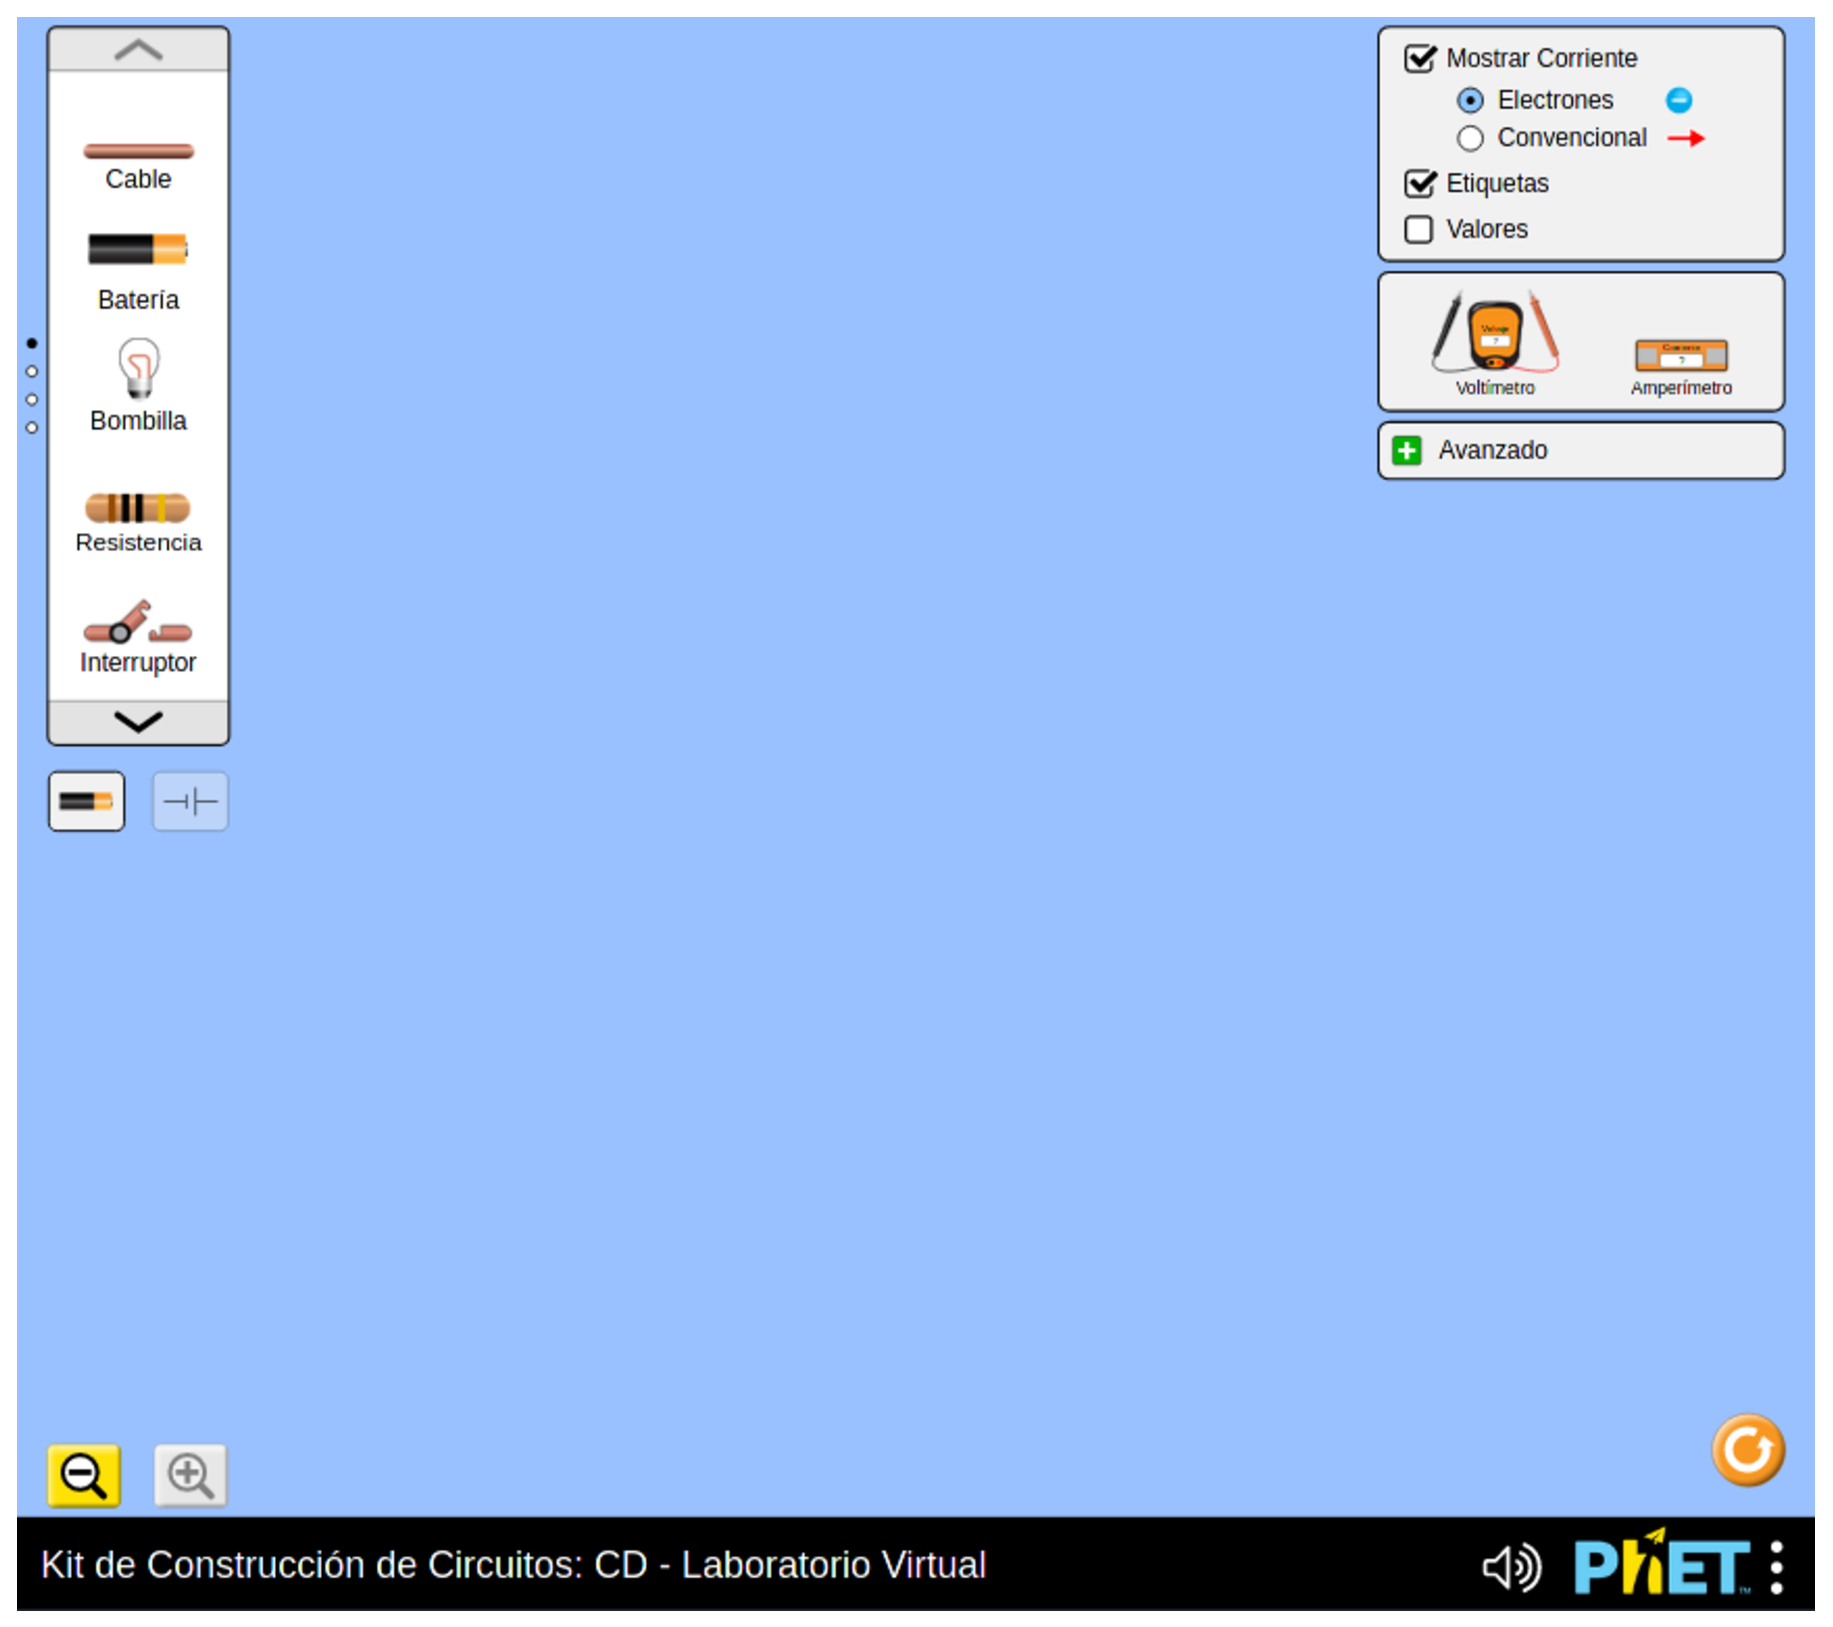
\includegraphics[scale=0.40]{resources/figura1.eps}
\caption{Simulador para el montaje de circuitos.}
\label{figura1}
\end{figure}

\item Fijar un valor constante de la resistencia eléctrica, y armar el circuito
de la \textbf{Figura \ref{figura2}}.

\begin{figure}[!h]
\centering
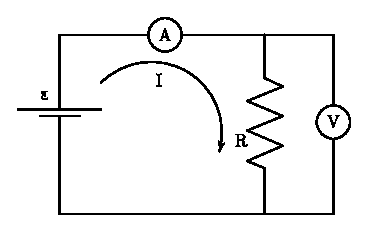
\includegraphics[scale=1.00]{resources/figura2.eps}
\caption{Circuito para la medición de la ley de \emph{Ohm}.}
\label{figura2}
\end{figure}

\item Para un voltaje en la resistencia, registrar la corriente que circula por
ella.
\item Variar el voltaje en la resistencia, y registrar el cambio respectivo en
la corriente eléctrica.
\item Registrar las mediciones tomadas, elaborar las gráficas e interpretar los
resultados.
\end{enumerate}

\subsection{Fuentes de tensión continua}
A continuación se describe el procedimiento experimental que se llevará a cabo.

\begin{enumerate}
\item Ir al simulador ubicado en la dirección web:
(https://phet.colorado.edu/sims/html/circuit-construction-kit-dc-virtual-lab/latest/circuit-construction-kit-dc-virtual-lab\_es.html),
tal como se muestra en la \textbf{Figura \ref{figura1}}.

\item Fijar un valor constante de la resistencia eléctrica, y armar el circuito
de la \textbf{Figura \ref{figura3}}.

\begin{figure}[!h]
\centering
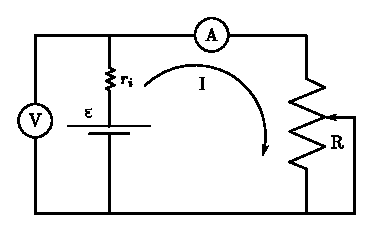
\includegraphics[scale=1.00]{resources/figura3.eps}
\caption{Circuito para la medición de tensión continua.}
\label{figura3}
\end{figure}

\item Fijar un valor constante de voltaje de la fuente.
\item Variar el valor de la resistencia, y registrar el cambio respectivo en la
    corriente eléctrica y el voltaje del circuito.
\item Registrar las mediciones tomadas, elaborar las gráficas e interpretar los
resultados.
\end{enumerate}

\section{Resultados}

\subsection{Ley de \emph{Ohm}}
En la \textbf{Figura \ref{figura4}} puede verse el montaje del circuito
realizado para la toma de datos.

\begin{figure}[!h]
\centering
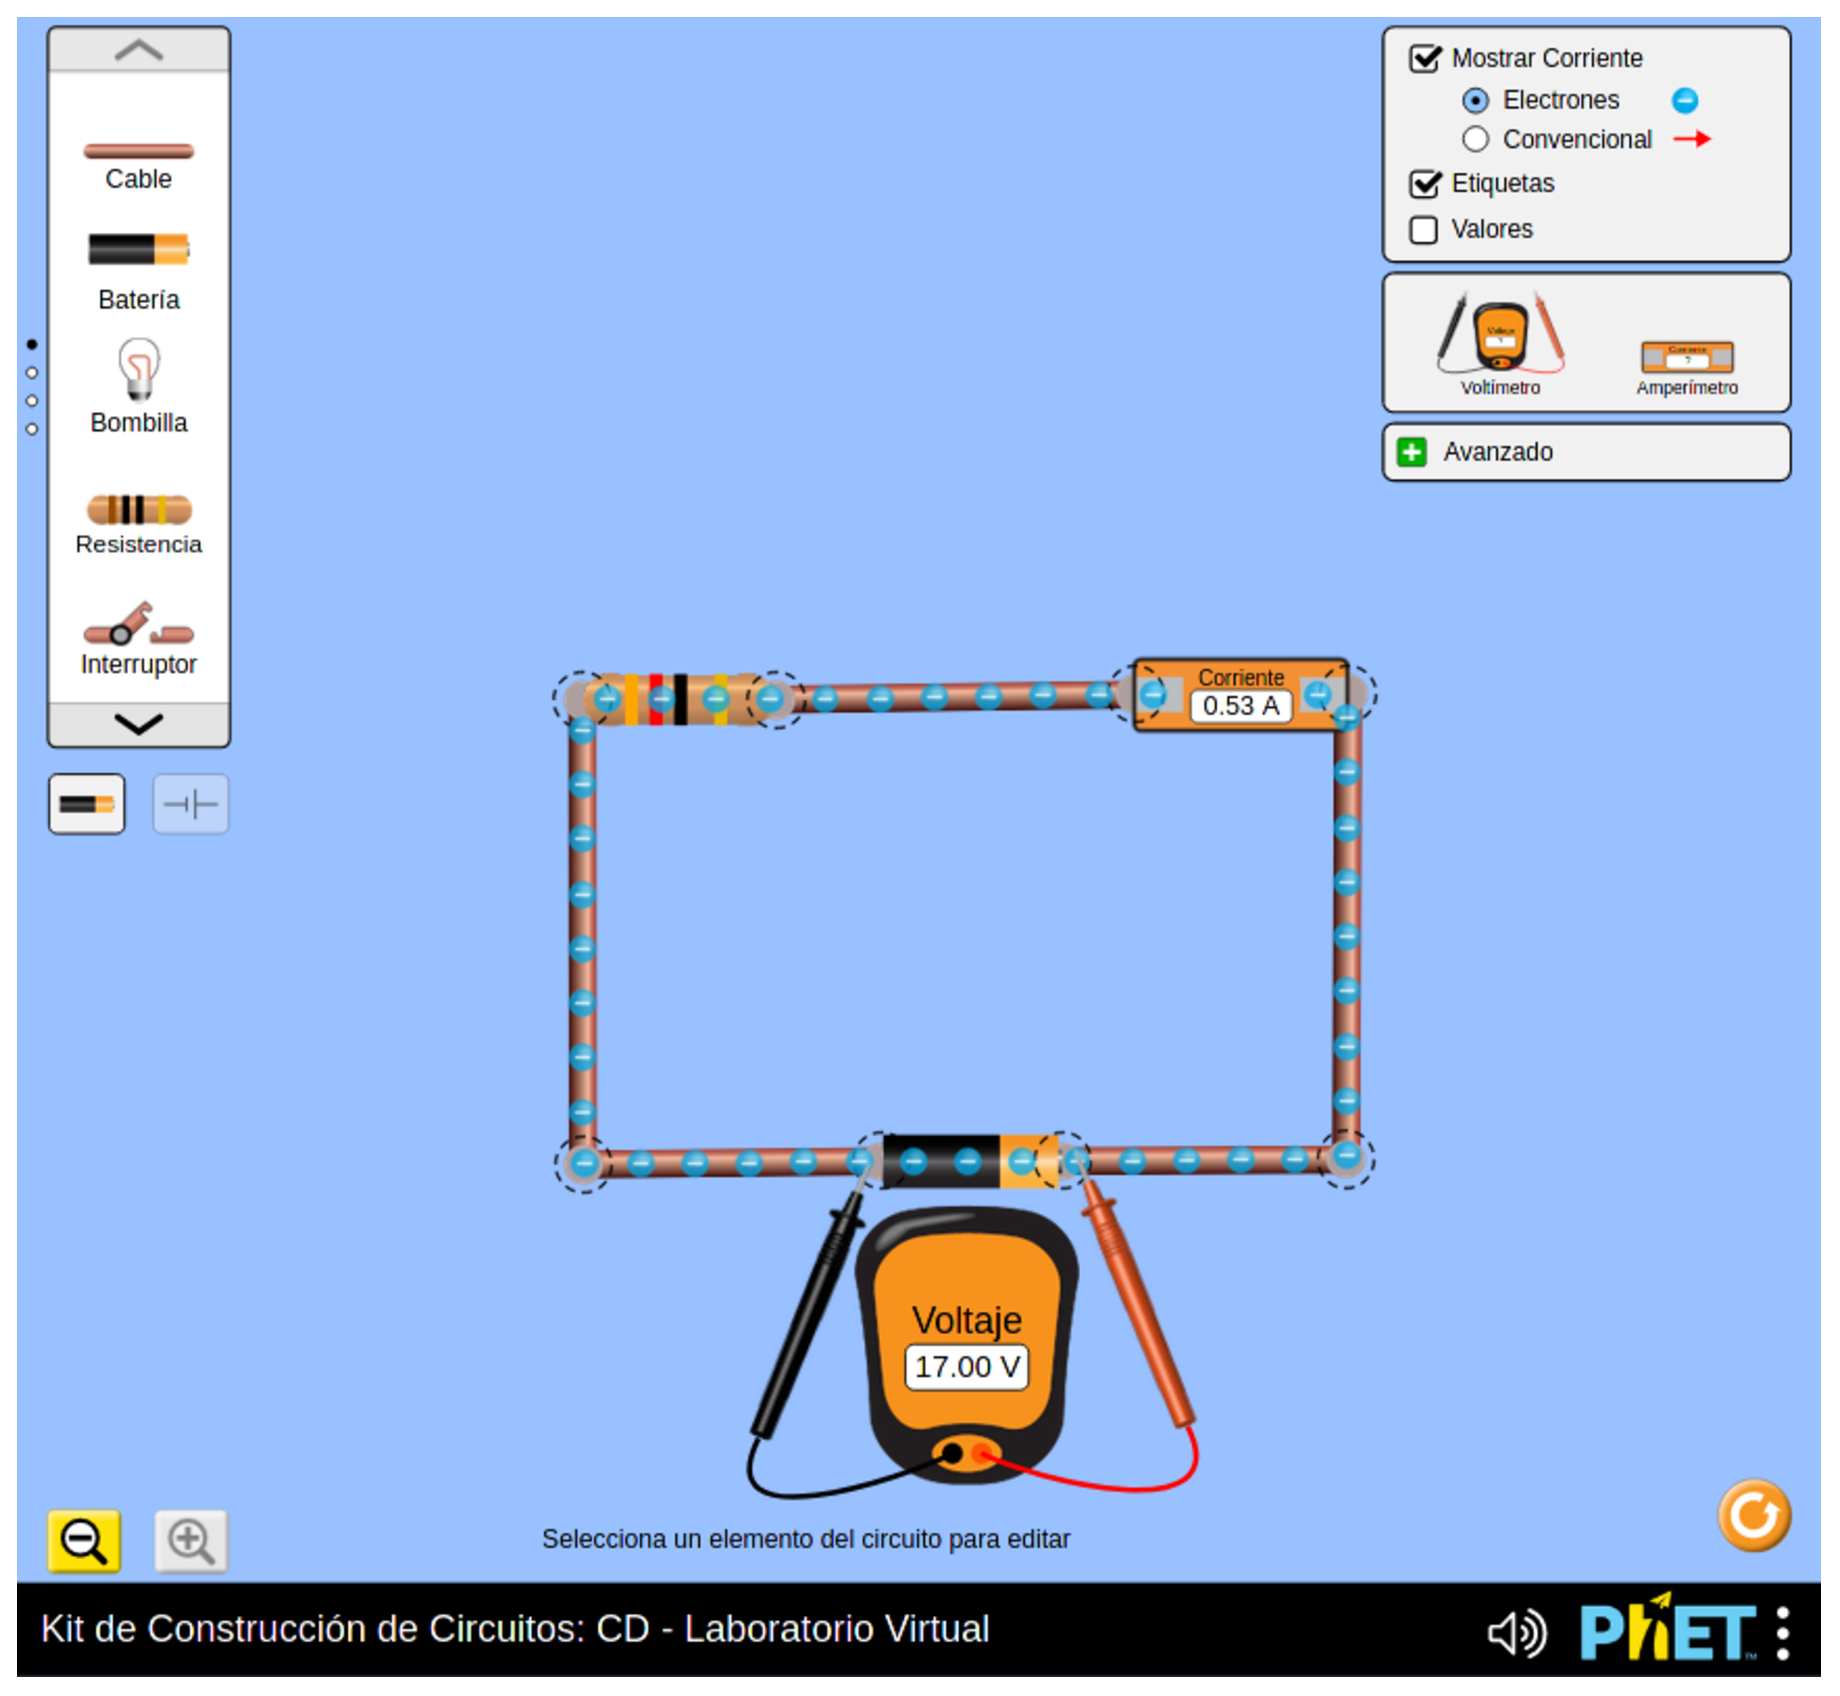
\includegraphics[scale=0.40]{resources/figura4.eps}
\caption{Simulador para la medición de la ley de \emph{Ohm}.}
\label{figura4}
\end{figure}

Valor de la resistencia:

\begin{equation*}
    R = 32 [\Omega]
\end{equation*}

En el \textbf{Cuadro \ref{cuadro1}} se presentan los valores de la intensidad de
corriente eléctrica ($I$) para diferentes valores de voltaje ($V$).

\begin{table}[!h]
\begin{center}
\begin{tabular}{|c|>{\centering}m{2.0cm}<{\centering}
                  |>{\centering}m{2.0cm}<{\centering}|}
\hline
$i$ & $I_i [A]$ & $V_i [V]$ \tabularnewline \hline
1 & 0.16 &  5.0 \tabularnewline \hline
2 & 0.34 & 11.0 \tabularnewline \hline
3 & 0.66 & 21.0 \tabularnewline \hline
4 & 0.94 & 30.0 \tabularnewline \hline
5 & 1.25 & 40.0 \tabularnewline \hline
6 & 1.62 & 52.0 \tabularnewline \hline
7 & 2.06 & 66.0 \tabularnewline \hline
8 & 2.66 & 85.0 \tabularnewline \hline
\end{tabular}
\caption{Mediciones de la corriente eléctrica para diferentes voltajes.}
\label{cuadro1}
\end{center}
\end{table}

A partir de los datos del \textbf{Cuadro \ref{cuadro1}}, se obtiene la gráfica
presentada en la \textbf{Figura \ref{figura5}}.

\begin{figure}[!h]
\centering
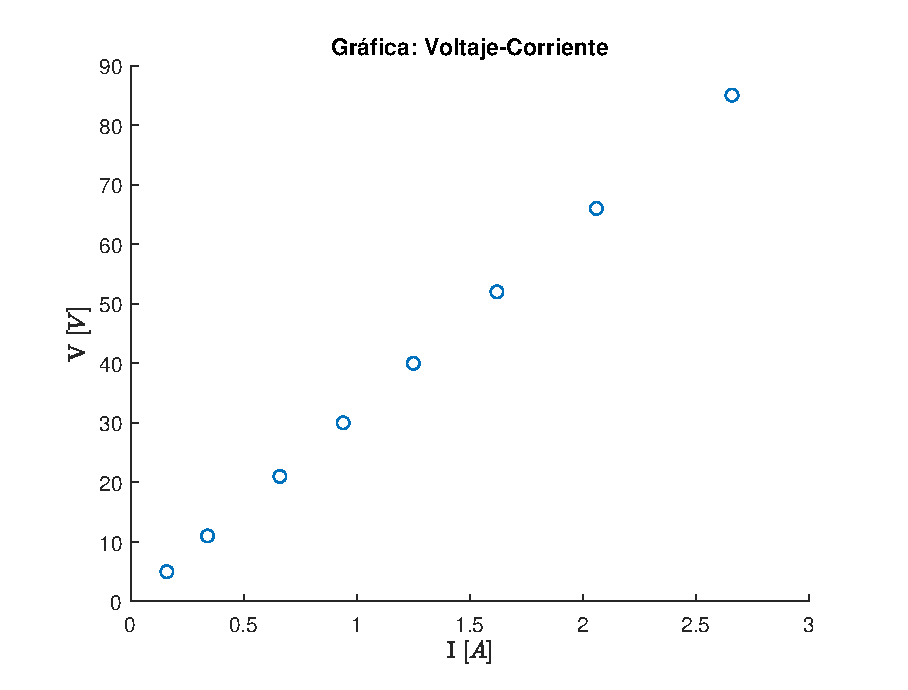
\includegraphics[scale=0.75]{resources/p1.eps}
\caption{Voltaje en función de la corriente eléctrica para una resistencia
    constante.}
\label{figura5}
\end{figure}

Por tanto, la ecuación de ajuste es:

\begin{equation*}
    V = A + B \cdot I
\end{equation*}

Calculamos los parámetros de la recta por el método de los mínimos cuadrados,
con la ayuda de los datos presentados en el \textbf{Cuadro \ref{cuadro2}}.

\begin{table}[!h]
\begin{center}
\begin{tabular}{|c|>{\centering}m{1.5cm}<{\centering}
                  |>{\centering}m{1.6cm}<{\centering}
                  |>{\centering}m{1.6cm}<{\centering}
                  |>{\centering}m{1.6cm}<{\centering}
                  |>{\centering}m{2.2cm}<{\centering}
                  |>{\centering}m{2.2cm}<{\centering}|}
\hline
$i$ & $I_i V_i$ & $I^2_i$ & $V^2_i$ & $Y$ & $d_i$ & $d^2_i$ \tabularnewline \hline
1 &   0.8000 & 0.0256 &   25 &  5.0961 & -0.0961 & 0.0092 \tabularnewline \hline
2 &   3.7400 & 0.1156 &  121 & 10.8585 &  0.1415 & 0.0200 \tabularnewline \hline
3 &  13.8600 & 0.4356 &  441 & 21.1027 & -0.1027 & 0.0106 \tabularnewline \hline
4 &  28.2000 & 0.8836 &  900 & 30.0664 & -0.0664 & 0.0044 \tabularnewline \hline
5 &  50.0000 & 1.5625 & 1600 & 39.9905 &  0.0095 & 0.0001 \tabularnewline \hline
6 &  84.2400 & 2.6244 & 2704 & 51.8354 &  0.1646 & 0.0271 \tabularnewline \hline
7 & 135.9600 & 4.2436 & 4356 & 65.9212 &  0.0788 & 0.0062 \tabularnewline \hline
8 & 226.1000 & 7.0756 & 7225 & 85.1291 & -0.1291 & 0.0167 \tabularnewline \hline
\end{tabular}
\caption{Valores para el método de mínimos cuadrados.}
\label{cuadro2}
\end{center}
\end{table}

\begin{equation*}
    n = 8
\end{equation*}
\begin{equation*}
    \sum I_i = 9.6900
\end{equation*}
\begin{equation*}
    \sum V_i = 310
\end{equation*}
\begin{equation*}
    \sum I^2_i = 16.9665
\end{equation*}
\begin{equation*}
    \sum V^2_i = 17372
\end{equation*}
\begin{equation*}
    \sum I_i V_i = 542.9000
\end{equation*}
\begin{equation*}
    \Delta_1 = n \sum I^2_i - \left( \sum I_i \right)^2 = 41.8359
\end{equation*}
\begin{equation*}
    \Delta_2 = n \sum V^2_i - \left( \sum V_i \right)^2 = 42876
\end{equation*}
\begin{equation*}
    A = \frac{\sum V_i \sum I^2_i - \sum I_i V_i \sum I_i}{\Delta_1} = -0.0260
\end{equation*}
\begin{equation*}
    B = \frac{n \sum I_i V_i - \sum I_i \sum V_i}{\Delta_1} = 32.0132
\end{equation*}
\begin{equation*}
    \sum d^2 = 0.0943
\end{equation*}
\begin{equation*}
    \sigma^2 = \frac{\sum d^2_i}{n-2} = 0.0157
\end{equation*}
\begin{equation*}
    \sigma_A = \sqrt{\frac{\sigma^2 \sum d^2_i}{\Delta_1}} = 0.0798
\end{equation*}
\begin{equation*}
    \sigma_B = \sqrt{\frac{\sigma^2 n}{\Delta_1}} = 0.0548
\end{equation*}

\begin{equation*}
    A = (-0.03 \pm 0.08)[V]; 307.54 \%
\end{equation*}
\begin{equation*}
    B = (32.01 \pm 0.05)[\Omega]; 0.17 \%
\end{equation*}

Siendo el coeficiente de correlación:

\begin{equation*}
    r = \frac{n \sum I_i V_i - (\sum I_i)(\sum V_i)}{\sqrt{\Delta_1 \Delta_2}} = 1.0000
\end{equation*}

La ecuación de la recta resultante es:

\begin{equation*}
    V = -0.03 + 32.01 \cdot I
\end{equation*}

Despreciando el valor de $A$ y utilizando la ley de \emph{Ohm}, se determina el
valor de la resistencia eléctrica:

\begin{center}
\begin{tabular}{|>{\centering}m{11.0cm}<{\centering}|}
\hline
\textbf{Resultado}
\tabularnewline \hline
\\
$R = (32.01 \pm 0.05) [\Omega]; 0.17 \%$ \tabularnewline
\\
\hline
\end{tabular}
\end{center}

\subsection{Fuentes de tensión continua}
En la \textbf{Figura \ref{figura6}} puede verse el montaje del circuito
realizado para la toma de datos.

\begin{figure}[!h]
\centering
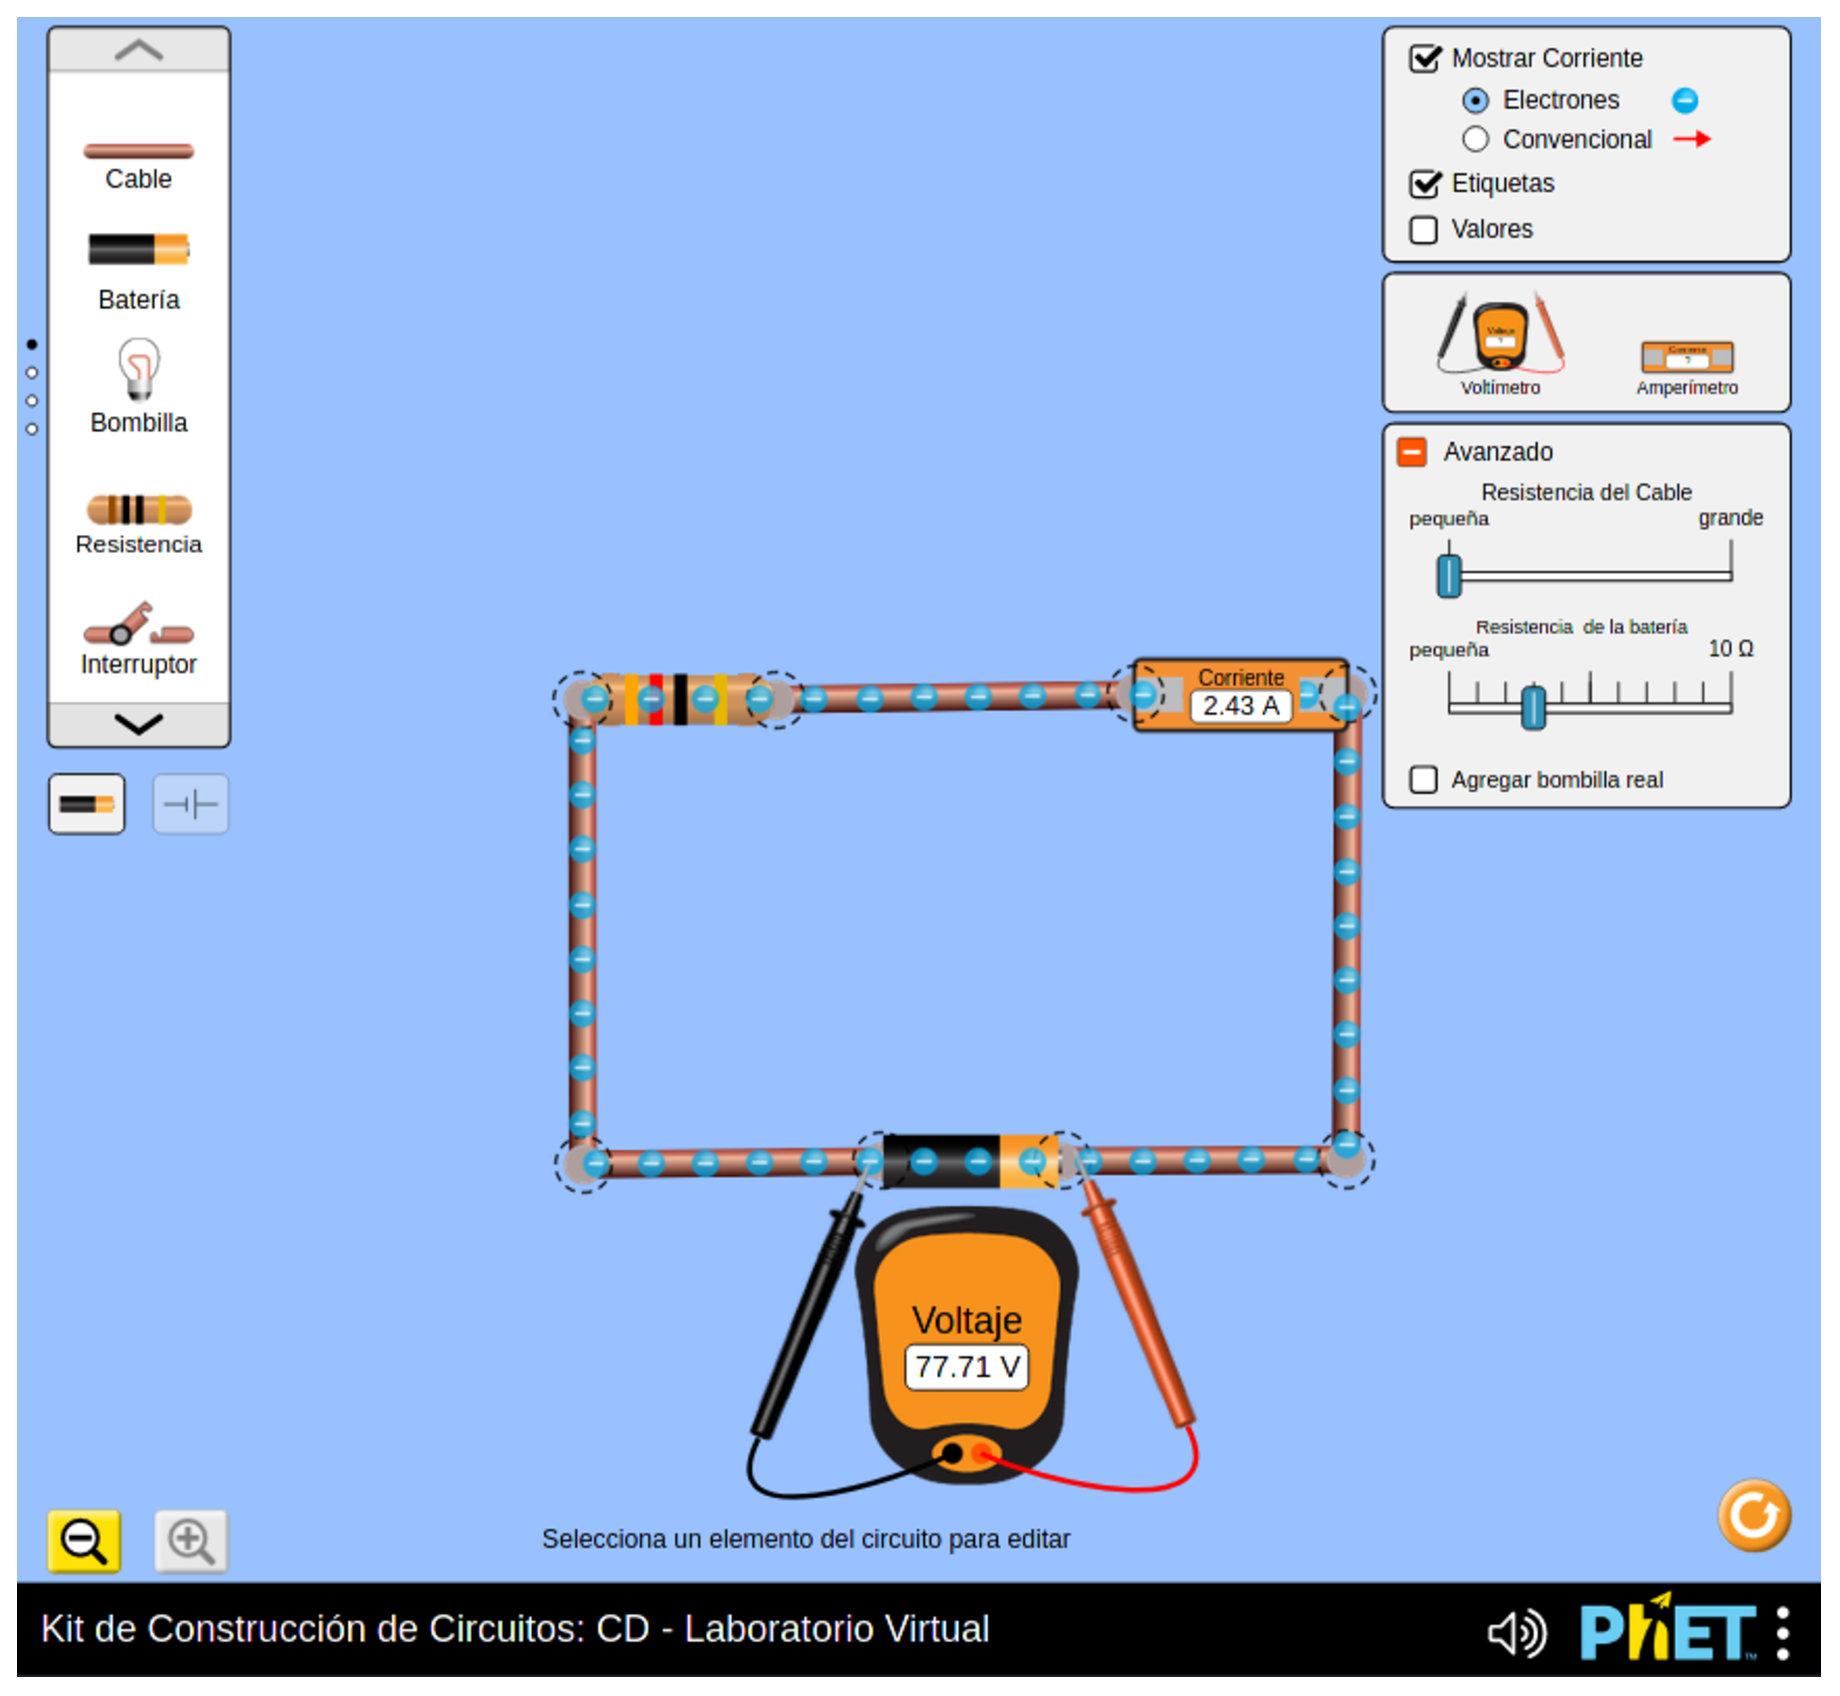
\includegraphics[scale=0.40]{resources/figura6.eps}
\caption{Simulador para la medición de tensión continua.}
\label{figura6}
\end{figure}

Valor de la resistencia interna:

\begin{equation*}
    R_i = 10 [\Omega]
\end{equation*}

En el \textbf{Cuadro \ref{cuadro3}} se presentan los valores de la intensidad de
corriente eléctrica ($I$) para diferentes valores de voltaje ($V$).

\begin{table}[!h]
\begin{center}
\begin{tabular}{|c|>{\centering}m{2.0cm}<{\centering}
                  |>{\centering}m{2.0cm}<{\centering}|
                  |>{\centering}m{2.0cm}<{\centering}|}
\hline
$i$ & $I_i [A]$ & $V_i [V]$ & $R_i [\Omega]$ \tabularnewline \hline
1 & 9.44 & 56.67 &   6.0 \tabularnewline \hline
2 & 8.50 & 59.50 &   7.0 \tabularnewline \hline
3 & 7.08 & 63.75 &   9.0 \tabularnewline \hline
4 & 5.31 & 69.06 &  13.0 \tabularnewline \hline
5 & 3.54 & 74.37 &  21.0 \tabularnewline \hline
6 & 2.12 & 78.62 &  37.0 \tabularnewline \hline
7 & 1.18 & 81.46 &  69.0 \tabularnewline \hline
8 & 0.69 & 82.93 & 120.0 \tabularnewline \hline
\end{tabular}
\caption{Mediciones de la corriente eléctrica para diferentes voltajes.}
\label{cuadro3}
\end{center}
\end{table}

A partir de los datos del \textbf{Cuadro \ref{cuadro3}}, se obtiene la gráfica
presentada en la \textbf{Figura \ref{figura7}}.

\begin{figure}[!h]
\centering
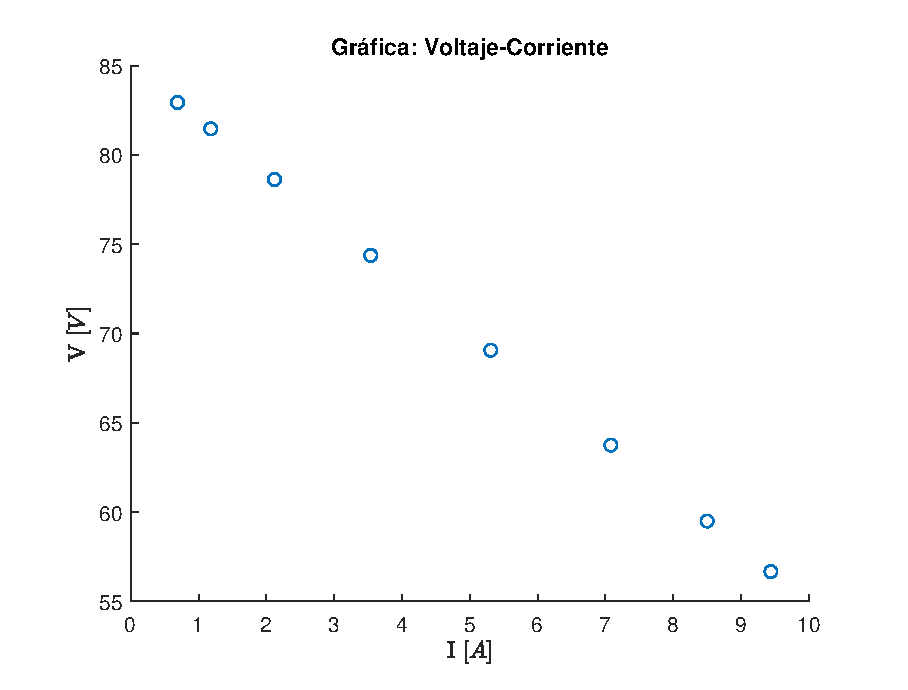
\includegraphics[scale=0.75]{resources/p3.eps}
\caption{Voltaje en función de la corriente eléctrica para una fuente de
    tensión.}
\label{figura7}
\end{figure}

Por tanto, la ecuación de ajuste es:

\begin{equation*}
    V_{ab} = A + B \cdot I
\end{equation*}

Calculamos los parámetros de la recta por el método de los mínimos cuadrados,
con la ayuda de los datos presentados en el \textbf{Cuadro \ref{cuadro4}}.

\begin{table}[!h]
\begin{center}
\begin{tabular}{|c|>{\centering}m{1.4cm}<{\centering}
                  |>{\centering}m{1.4cm}<{\centering}
                  |>{\centering}m{2.4cm}<{\centering}
                  |>{\centering}m{1.4cm}<{\centering}
                  |>{\centering}m{1.8cm}<{\centering}
                  |>{\centering}m{3.0cm}<{\centering}|}
\hline
$i$ & $I_i V_i$ & $I^2_i$ & $V^2_i$ & $Y$ & $d_i$ & $d^2_i$ \tabularnewline \hline
1 & 534.9648 & 89.1136 & \num{3.2115e3} & 56.6718 & -0.0018 & \num{0.0032e-3} \tabularnewline \hline
2 & 505.7500 & 72.2500 & \num{3.5402e3} & 59.4919 &  0.0081 & \num{0.0652e-3} \tabularnewline \hline
3 & 451.3500 & 50.1264 & \num{4.0641e3} & 63.7521 & -0.0021 & \num{0.0046e-3} \tabularnewline \hline
4 & 366.7086 & 28.1961 & \num{4.7693e3} & 69.0624 & -0.0024 & \num{0.0058e-3} \tabularnewline \hline
5 & 263.2698 & 12.5316 & \num{5.5309e3} & 74.3727 & -0.0027 & \num{0.0072e-3} \tabularnewline \hline
6 & 166.6744 &  4.4944 & \num{6.1811e3} & 78.6329 & -0.0129 & \num{0.1664e-3} \tabularnewline \hline
7 &  96.1228 &  1.3924 & \num{6.6357e3} & 81.4530 &  0.0070 & \num{0.0484e-3} \tabularnewline \hline
8 &  57.2217 &  0.4761 & \num{6.8774e3} & 82.9231 &  0.0069 & \num{0.0474e-3} \tabularnewline \hline
\end{tabular}
\caption{Valores para el método de mínimos cuadrados.}
\label{cuadro4}
\end{center}
\end{table}

\begin{equation*}
    n = 8
\end{equation*}
\begin{equation*}
    \sum I_i = 37.8600
\end{equation*}
\begin{equation*}
    \sum V_i = 566.3600
\end{equation*}
\begin{equation*}
    \sum I^2_i = 258.5806
\end{equation*}
\begin{equation*}
    \sum V^2_i = \num{4.0810 e4}
\end{equation*}
\begin{equation*}
    \sum I_i V_i = \num{2.4421 e3}
\end{equation*}
\begin{equation*}
    \Delta_1 = n \sum I^2_i - \left( \sum I_i \right)^2 = 635.2652
\end{equation*}
\begin{equation*}
    \Delta_2 = n \sum V^2_i - \left( \sum V_i \right)^2 = \num{5.7180 e3}
\end{equation*}
\begin{equation*}
    A = \frac{\sum V_i \sum I^2_i - \sum I_i V_i \sum I_i}{\Delta_1} = 84.9932
\end{equation*}
\begin{equation*}
    B = \frac{n \sum I_i V_i - \sum I_i \sum V_i}{\Delta_1} = -3.0002
\end{equation*}
\begin{equation*}
    \sum d^2 = \num{3.4814 e-4}
\end{equation*}
\begin{equation*}
    \sigma^2 = \frac{\sum d^2_i}{n-2} = \num{5.8023 e-5}
\end{equation*}
\begin{equation*}
    \sigma_A = \sqrt{\frac{\sigma^2 \sum d^2_i}{\Delta_1}} = 0.0049
\end{equation*}
\begin{equation*}
    \sigma_B = \sqrt{\frac{\sigma^2 n}{\Delta_1}} = \num{8.5481 e-4}
\end{equation*}

\begin{equation*}
    A = (84.993 \pm 0.005)[V]; 0.006 \%
\end{equation*}
\begin{equation*}
    B = (-3.0 \pm \num{8.5 e-4})[\Omega]; 0.03 \%
\end{equation*}

Siendo el coeficiente de correlación:

\begin{equation*}
    r = \frac{n \sum I_i V_i - (\sum I_i)(\sum V_i)}{\sqrt{\Delta_1 \Delta_2}} = -1.0000
\end{equation*}

La ecuación de la recta resultante es:

\begin{equation*}
    V_{ab} = 84.993 - 3.0 \cdot I
\end{equation*}

Utilizando la ley de voltaje de \emph{Kirchhoff}, se determina que el valor de
la $FEM$, resistencia interna y corriente de cortocircuito son:

\begin{center}
\begin{tabular}{|>{\centering}m{11.0cm}<{\centering}|}
\hline
\textbf{Resultado}
\tabularnewline \hline
\\
$\epsilon = (84.993 \pm 0.005) [V]; 0.006 \%$ \tabularnewline
\\
\hline
\end{tabular}
\end{center}

\begin{center}
\begin{tabular}{|>{\centering}m{11.0cm}<{\centering}|}
\hline
\textbf{Resultado}
\tabularnewline \hline
\\
$r_i = (-3.0 \pm \num{8.5 e-4}) [\Omega]; 0.03 \%$ \tabularnewline
\\
\hline
\end{tabular}
\end{center}

Se determinará la corriente de cortocircuito, a partir de la ecuación 
(\ref{icc}):

\begin{equation*}
    I_{cc} = \frac{\epsilon}{r_i} = 28.33 [A]
\end{equation*}

Las derivadas parciales son:

\begin{equation*}
    \frac{\partial{I_{cc}}}{\partial{\epsilon}} = \frac{1}{r_i}
\end{equation*}
\begin{equation*}
    \frac{\partial{I_{cc}}}{\partial{r_i}} = \frac{\epsilon}{r_i^2}
\end{equation*}

Siendo el error de la medición:

\begin{equation*}
    e_I = \sqrt{ \left(\frac{1}{r_i}\right)^2 \cdot e^2_\epsilon + \left(\frac{\epsilon}{r^2_i}\right)^2 \cdot e^2_r } = 0.008
\end{equation*}

Por tanto la corriente de cortocircuito es:

\begin{center}
\begin{tabular}{|>{\centering}m{11.0cm}<{\centering}|}
\hline
\textbf{Resultado}
\tabularnewline \hline
\\
$I_{cc} = (28.33 \pm 0.008) [A]; 0.03 \%$ \tabularnewline
\\
\hline
\end{tabular}
\end{center}

\end{document}

